\chapter{The LHC}
\section{Large Hadron Collider}
The Large Hadron Collider (LHC) is a circular synchrotron with a circumference
of \unit{27}{\kilo\meter}.
It has been constructed in the existing tunnel 
\unit{40-170}{\meter} beneath the border of France and Switzerland
that was previously home the LEP collider.

When operating at its design energy and luminosity it will collide beams or
protons at a centre of mass energy of \unit{14}{\TeV} and a luminosity of
\unit{$ 10^{34} $}{\rpsquare\cm\reciprocal\second} .
It is also designed to collide two \unit{5.5}{\TeV} beams of heavy ions, such
as lead nuclei.\cite{lhc}

The main motivation for the LHC is to determine the mechanism that is
responsible for electroweak symmetry breaking, of which the most favoured is the
Higgs mechanism.  The LHC was also designed to test the Standard Model at the
$\TeV$ scale at high precision and to search for new particles predicted by
theories beyond the standard model such as supersymmetric theories and theories
involving extra dimensions.  \FigureRef{fig:LHCxsec} shows various cross
sections for several physics processes as a function of the centre of mass
energy. The cross section for many physics processes of interest, such as the
Higgs cross section, are several orders of magnitude below the total inelastic
cross section and increase as a function of centre of mass energy.  The large
centre of mass energy and high luminosity of the LHC is needed to be able to
probe the small cross-sections of new physics processes of interest.

\begin{figure}[htbp]
  \centering
  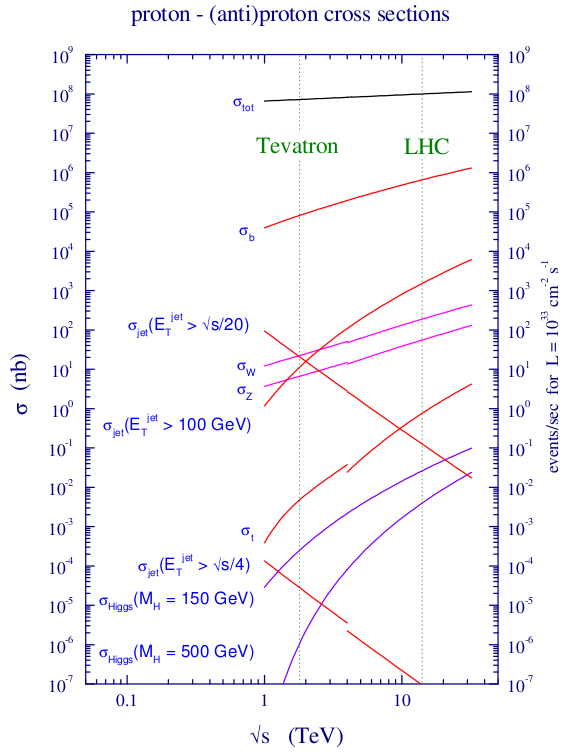
\includegraphics[width=0.8\textwidth]{xsec.png}
  \caption{The production cross sections as a function of centre of mass energy
for several Standard Model and new physics processes.}
  \label{fig:LHCxsec}
\end{figure}

The LHC is part of a larger accelerator complex as shown in figure
\FigureRef{fig:LHCcomplex}. Hydrogen gas is first ionised to produce a cloud of
protons, which are then accelerated by the LINAC2 linear accelerator to
\unit{50}{\MeV}.  Before being injected in to the Proton Synchrotron (PS) the
protons are injected in to the Proton Synchrotron Booster (PSB) and accelerated
to \unit{1.4}{\GeV}. In the PS the protons are formed in to bunches and the
energy is increased to \unit{25}{\GeV}. The bunches are then accelerated in the
Super Proton Synchrotron (SPS) to \unit{450}{\GeV} and then injected in to the
LHC.

%bunches?

\begin{figure}[htbp]
  \centering
  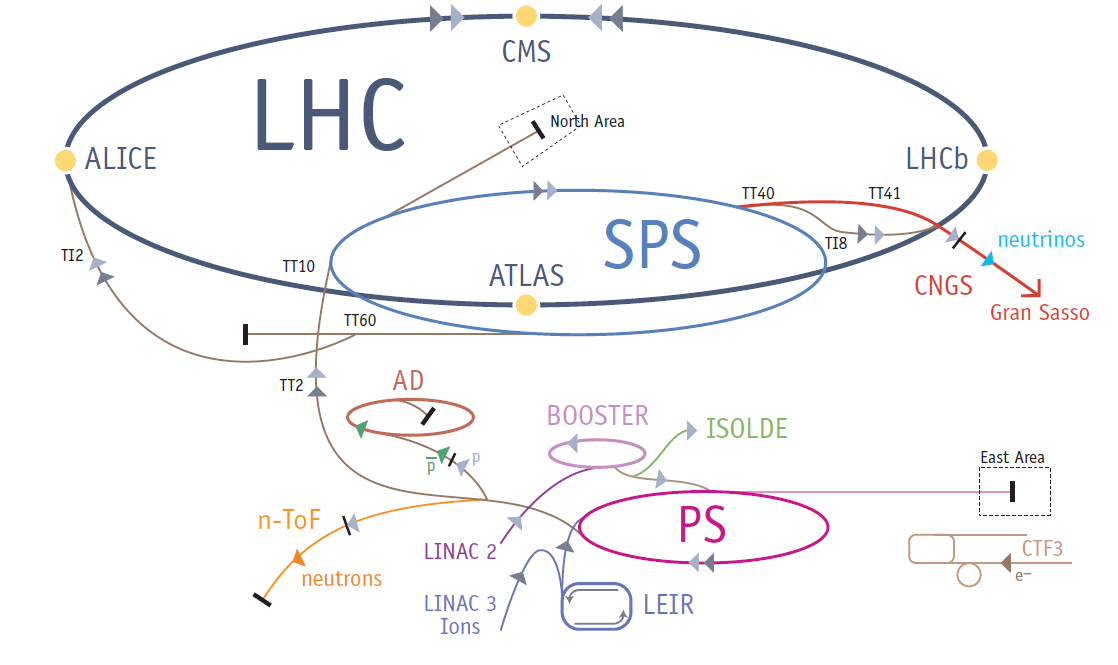
\includegraphics[width=0.8\textwidth]{accelerators.png}
  \caption{The LHC complex.}
  \label{fig:LHCcomplex}
\end{figure}

There are four main detector experiments studying the collisions at the LHC. 
ALICE (A Large Ion Collider Experiment) is designed to study the quark gluon
plasma that will be produced in the heavy ion collisions. 
LHCb (The Large Hadron Collider beauty) experiment is designed to study B-meson
decays to measure CP violation. 
ATLAS (A Toroidal LHC Apparatus) and CMS (Compact Muon Solenoid) are general
purpose detectors that are designed 
to search for a wide range of new physics.\cite{lhc}

\subsection{Operational History}
In September 2008 the LHC was commissioned and the first beams were circulated.
Before the first collisions could be delivered an interconnection
between two of the dipole magnets failed when the magnet quenched.
This led to a large amount to helium rapidly evaporating which caused
considerable damage to the machine.
Due to this incident it was decided that the LHC should be run at a lower centre
of mass energy of \unit{7}{\TeV} until the quench protection system could be
upgraded.

The LHC was repaired by the end of 2009 and the first collisions at a record
energy of \unit{2.36}{\TeV} were delivered in November. 
From March to November 2010 the LHC operated at \unit{7}{\TeV} delivering
\unit{46.4}{\invpb} of proton-proton collisions.
In November and October 2010 the LHC produced lead ion collisions at
\unit{2.36}{\TeV}.

\begin{figure}[htbp]
  \centering
  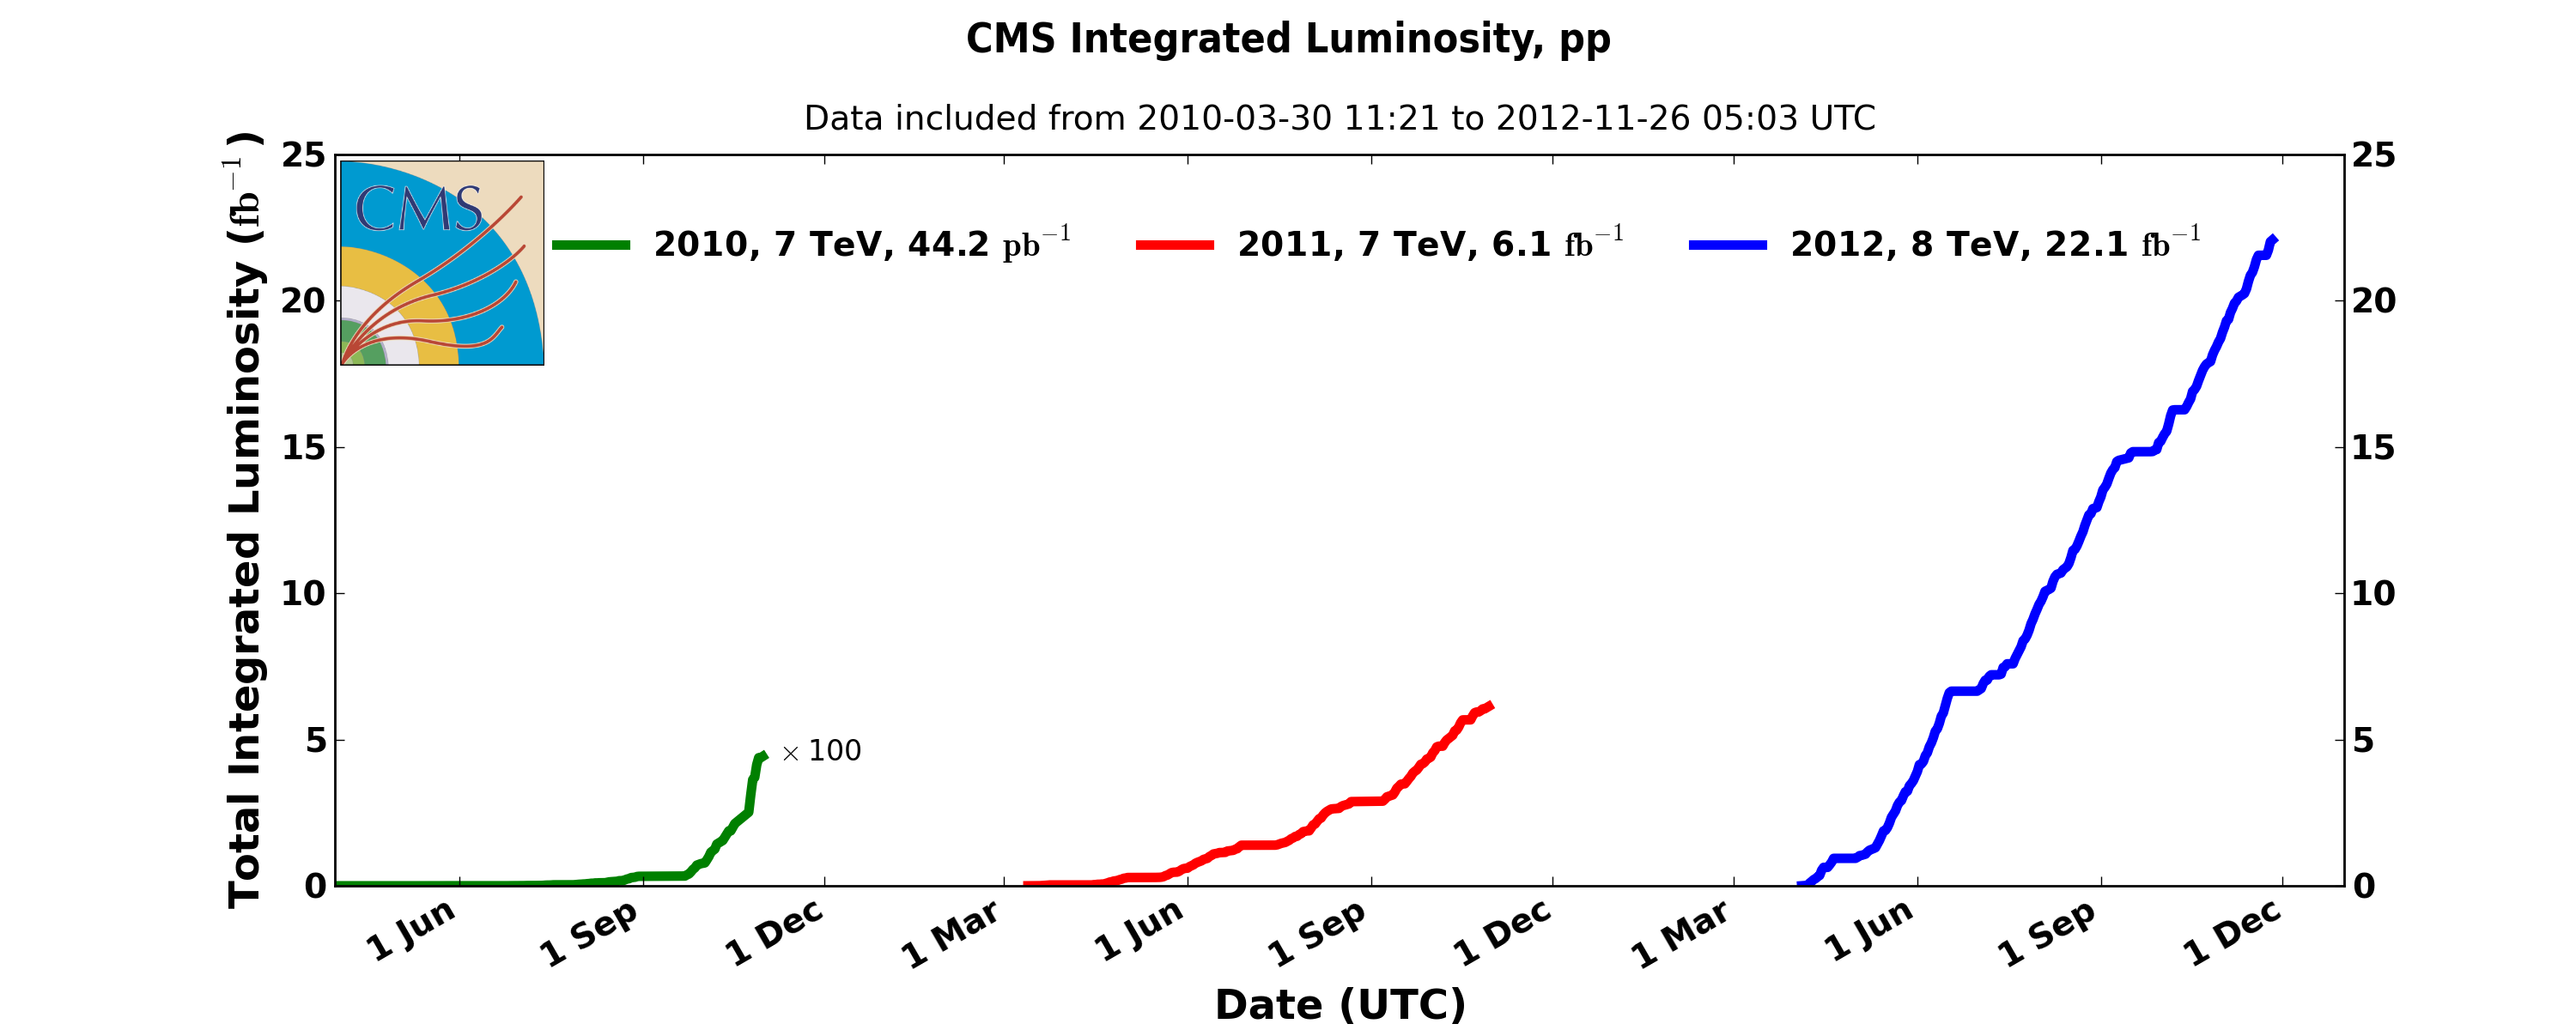
\includegraphics[width=\textwidth]{int_lumi_cumulative_pp_1.png}
  \caption{The luminosity delivered by LHC and recorded by CMS in 2010, 2011 and 2012}
  \label{fig:LHC2010}
\end{figure}


The target for running in 2011 was to deliver \unit{1}{\invfb} of data. This was
achieved by June. The target was increased to \unit{5}{\invfb} of data by the end
of the yeah which was achieved by October.
The luminosity delivered by LHC and recorded in CMS in 2010, 2011 and 2012 is
shown in \FigureRef{fig:LHC2010}.

\section{CMS Detector}
CMS (Compact Muon Solenoid) is one of the two general purpose
detectors designed to study LHC collisions. 

% The goals of the LHC physics program are to search for the Higgs, SUSY etc

The design goals of the CMS detector are:\cite{tdr}

\begin{itemize}
  \item Good muon identification and momentum resolution and the ability to
unambiguously assign charge to muons with $\PT < \unit{1}{\TeV}$
  \item Good charged particle momentum resolution and reconstruction in the
tracker.
  \item Good electromagnetic energy resolution. 
  \item Good \ETmiss and dijet mass resolution.
\end{itemize}

The design of CMS meets these requirements while overcoming significant
experimental challenges.  At design luminosity, $\approx 1 $ billion inelastic
events will occur in CMS every second, where as CMS is limited to storing the
data of only $\approx 100 $ events can be stored.  The detector must be able to
reduce this rate with a trigger to accept events that are interesting from a
physics perspective and reject events otherwise.

In addition to this challenge each event of interest will have on average 20
inelastic events superimposed on it. This results in around 1000 charged
particles produced every \unit{25}{\ns}, which will require the detectors to
have a high granularity with a good time resolution to ensure a low occupancy.
The large flux of particles will also produce high radiation levels which will
require radiation hard detectors and electronics.

\begin{figure}[htbp]
  \centering
  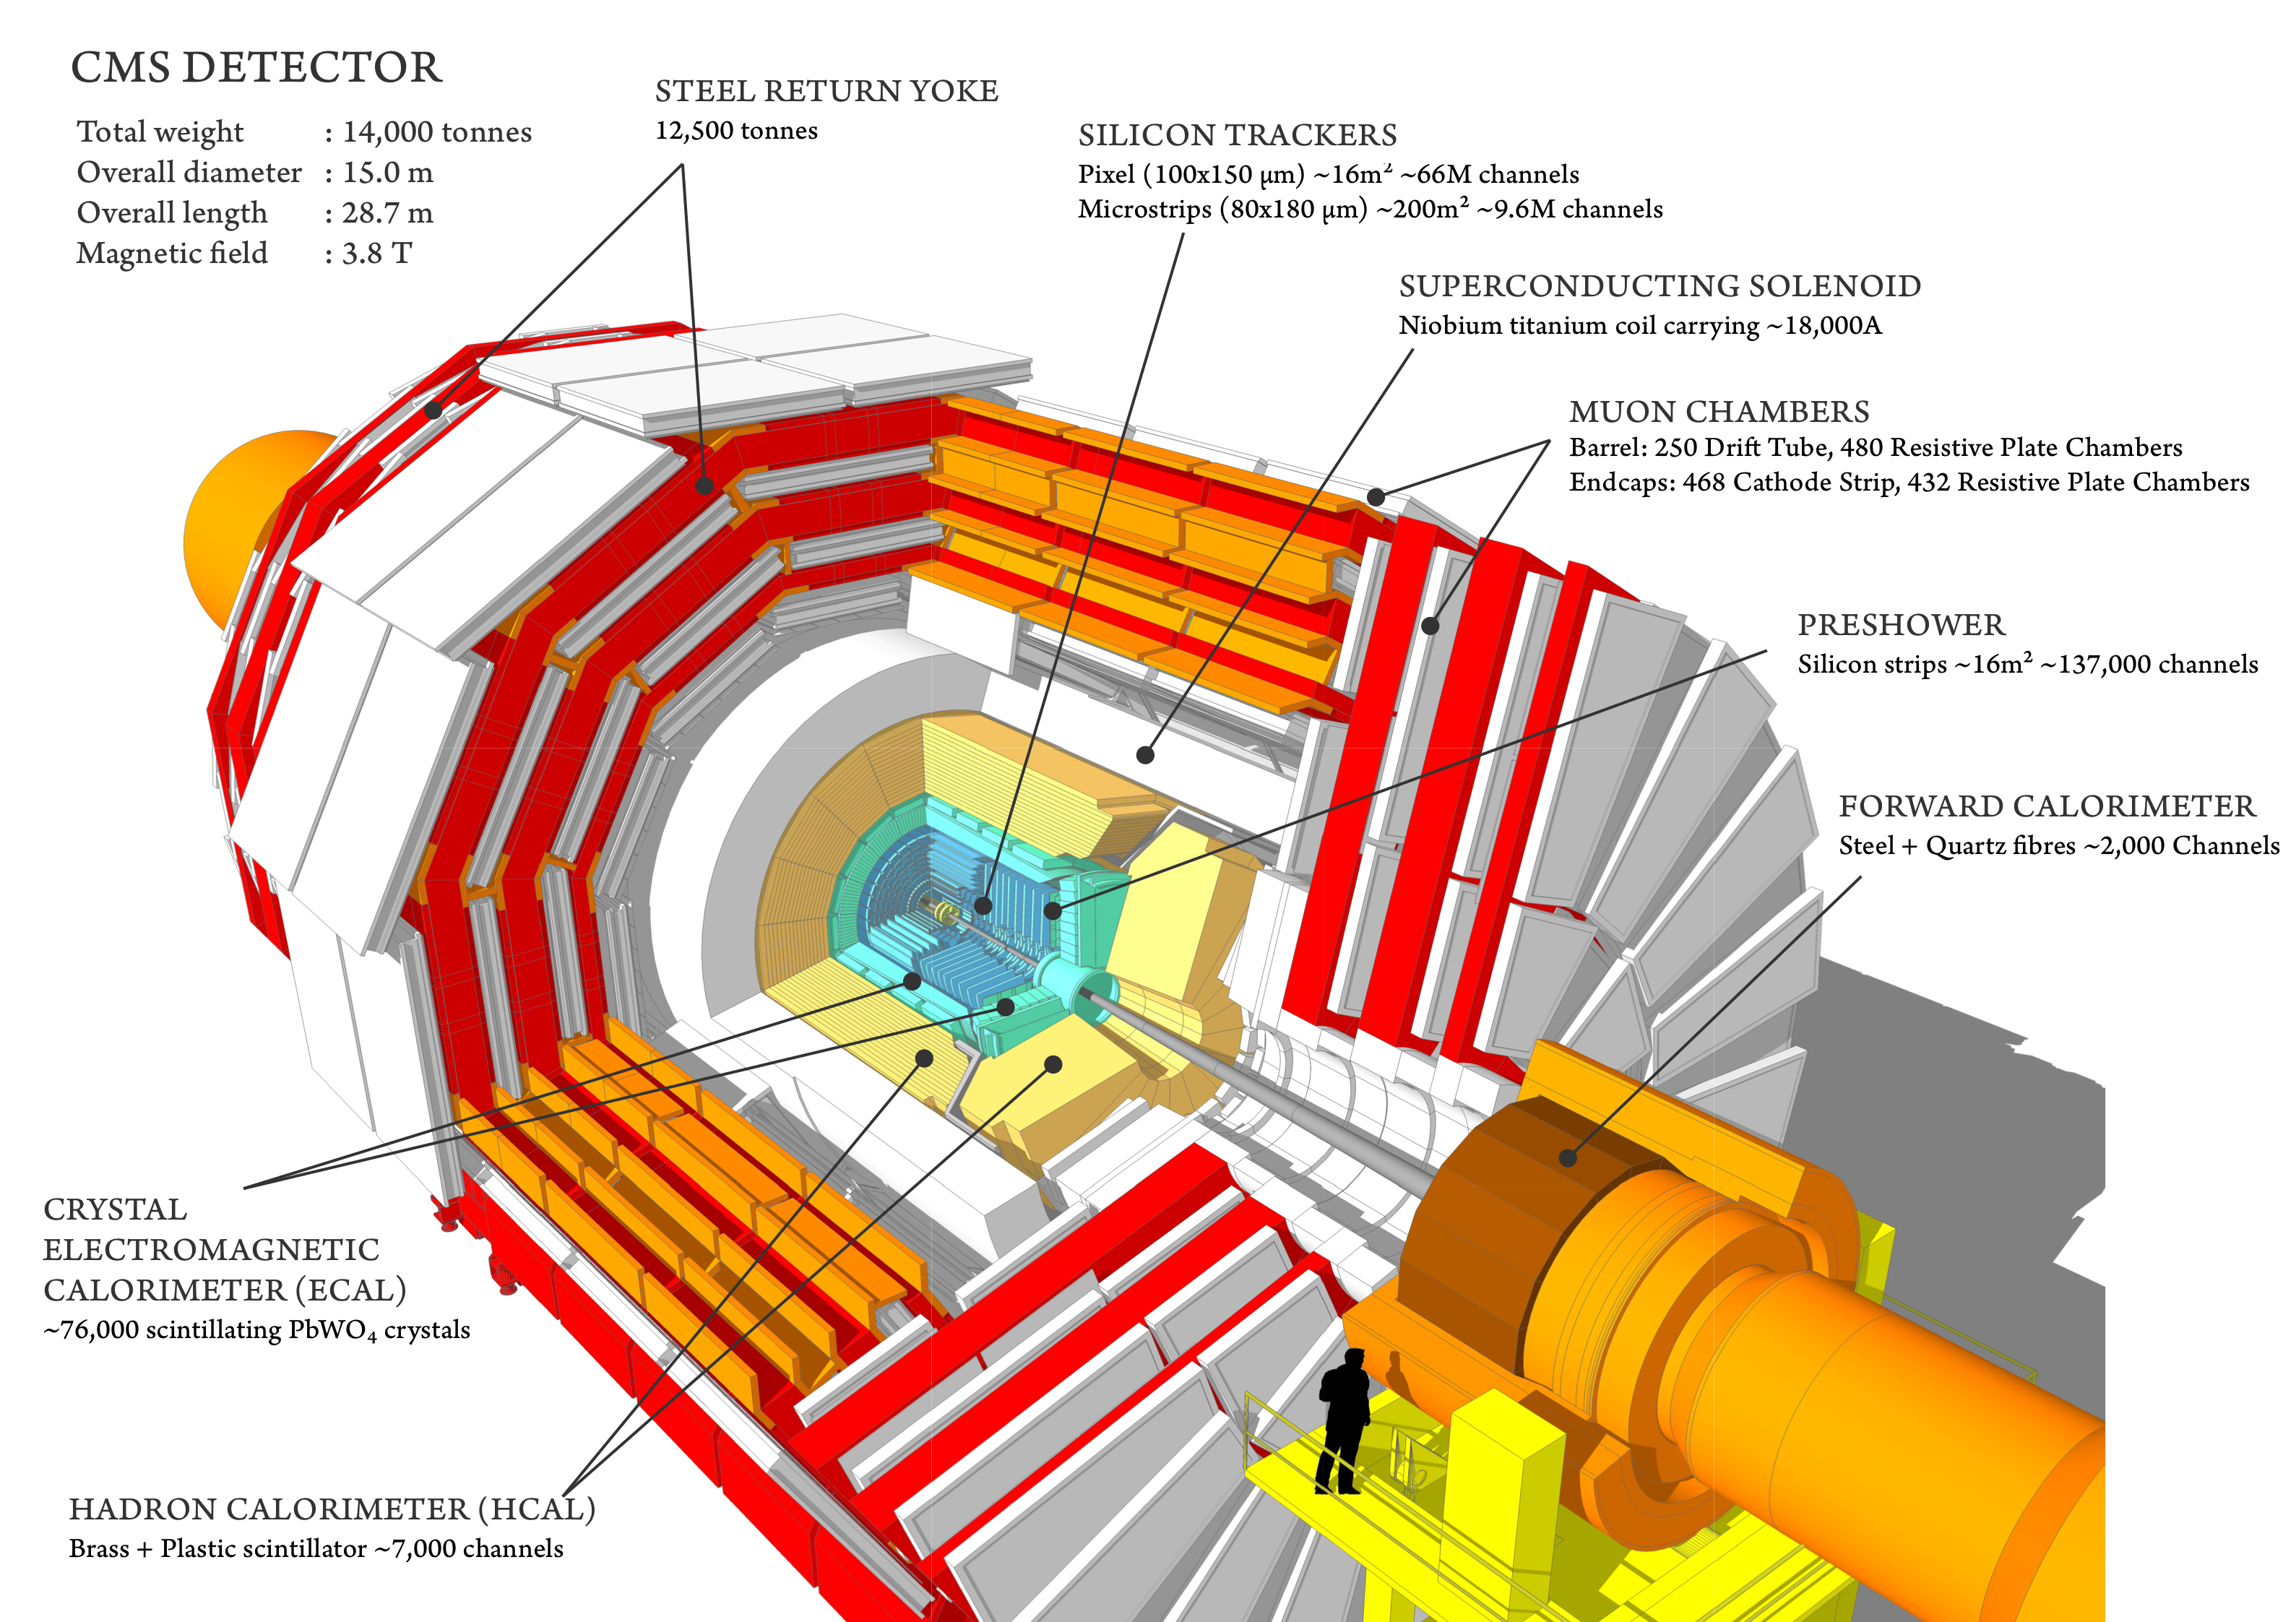
\includegraphics[width=0.8\textwidth]{cms_su.png}
  \caption{Diagram of the CMS detector, from\cite{sketchup}.}
  \label{fig:CMSnc}
\end{figure}

An overview of the detector is shown in \FigureRef{fig:CMSnc}.  Starting at the
interaction point in the centre of the detector and moving radially outwards,
CMS comprises the pixel tracker, silicon tracker, lead-tungstate ECAL, sampling
brass-plate HCAL, \unit{4}{\tesla} superconducting solenoid magnet, an outer
HCAL and four muon chambers.

\subsection{Magnet}
A large superconducting solenoid provides the basis for the design of the CMS
detector, and is the main structural support for the detector components in the
barrel region.

The superconducting magnet in CMS produces a \unit{4}{\tesla} field in a bore of
\unit{6}{\meter} diameter and \unit{12.5}{\meter} length.  While operating at
full current the magnet stores \unit{2.6}{\giga\joule} of energy.  A large
magnetic field is needed to give CMS a large bending power and the ability to
precisely measure the momentum of high-energy charged particles.  The solenoid
bore is large enough that the tracking detectors and the calorimetry can fit
inside it.\cite{cms}

The magnetic flux is returned through a \unit{1.8}{\meter} thick saturated iron
yoke which is interleaved with the muon detector.

\subsection{Tracking}
The inner tracker is designed to accurately and efficiently measure the
trajectories of charged particles produced in collisions at the centre of CMS.
The tracker is also required to be able to reconstruct secondary vertices caused
by the decay of a long lived particle.  At the design luminosity of the LHC it
is expected that every \unit{25}{\ns} an average of 1000 particles will traverse
the inner detector therefore it is required that the inner tracker has a high
granularity and a fast response while remaining resilient to radiation damage. 

\begin{figure}[htbp]
  \centering
  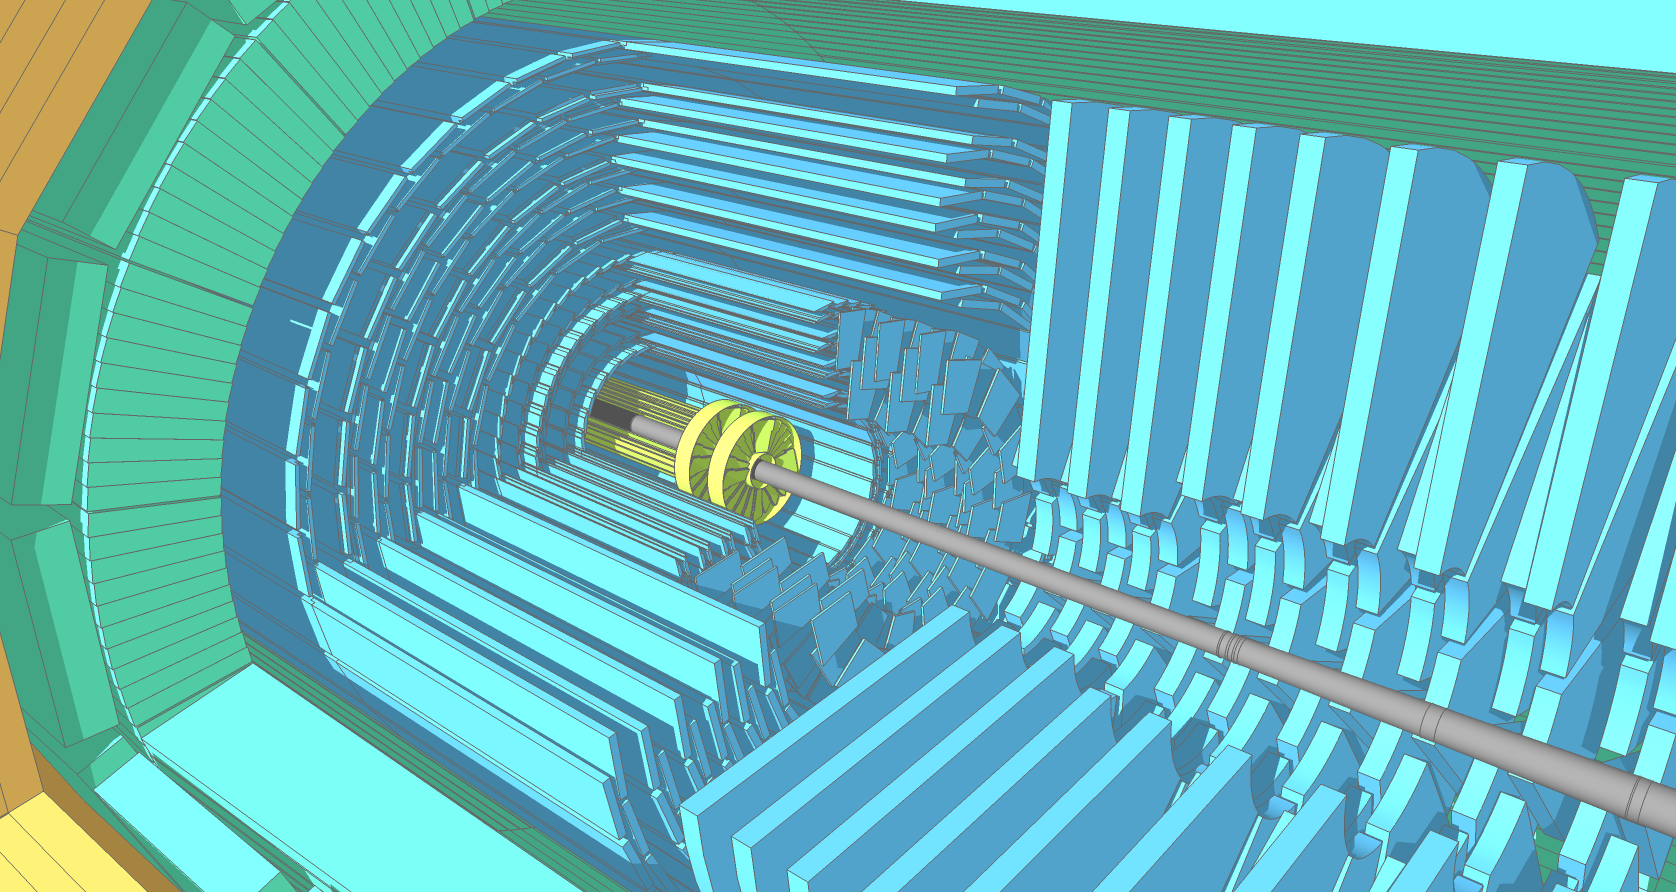
\includegraphics[width=0.8\textwidth]{strip.png}
  \caption{Close up of the CMS inner tracker. The pixel tracker is shown in lime
and the microstrip detector is show in blue.\cite{sketchup} }
  \label{fig:tracker}
\end{figure}

A close up view of the inner tracker is shown in \FigureRef{fig:tracker}.  The
tracker utilises silicon pixel detectors in the inner most layers where the
particle flux is the highest.  Outside of the pixel detector, the tracking
detector comprises several layers of silicon microstrip detectors where the
particle flux is reduced.  The total active area of silicon in the CMS tracker
is over \unit{200}{\meter\squared}.\cite{cms}

\subsubsection{Pixel Tracker}
The pixel tracker consists of three layers of hybrid silicon pixel detectors in
the barrel region and two in the endcap region. 
The barrel layers are positioned at radii 4.4, 7.3 and \unit{10.2}{\cm} and have
a length of \unit{53}{\cm}. The two layers in the endcap are located at
$|z|=34.5$ and \unit{46.5}{\cm} with an inner radius of \unit{6}{\cm} and an
outer radius of \unit{15}{\cm}.

Each pixel has a surface area of \unit{$100\times150$}{\micron} which results in
an average particle density of $\mathcal{O}(10^{-4})$ per crossing.

\subsubsection{Strip Tracker}
The strip tracker is split in to two regions according to the particle flux. In
the region \unit{$20<r<55$}{cm} microstrip detectors with a cell size of
$\unit{10}{\cm}\times\unit{80}{\micron}$ are used with an average occupancy of
$\approx\unit{2-3}{\%}$.
Outside this the flux is low enough to allow for the use of larger pitch silicon
microstrips with a cell size of $\unit{25}{\cm}\times\unit{180}{\micron}$ with
an average occupancy of $\approx\unit{1}{\%}$.
The silicon entire silicon strip detector consists of approximately 15400
modules.

The barrel strip tracker comprises two parts, the inner (TIB) and outer (TOB)
trackers. The TIB and TOB are formed of 4 and 6 layers respectively.

The endcaps are separated in to the Tracker End Cap (TEC) and the Tracker Inner
Disks (TID). The TEC is split in to nine disks and covers the region
$\unit{1200}{\mm} < |Z| < \unit{2800}{\mm}$. The TID comprises three rings
and fills the gap between the TEC and the TIB.

\subsection{Electromagnetic Calorimetry}
The electromagnetic calorimeter (ECAL) is 
designed to measure the energy of
particles with a high resolution and granularity.
A close up view of the CMS calorimetry is shown in \FigureRef{fig:calo}, where the
ECAL is shown in green.
It is a hermetic, homogeneous calorimeter comprising 61200 individual lead
tungstate ($PbWO_{4}$) scintillation crystals in the barrel region
($|\eta|<1.479$) closed by 7324 crystals in each of the two endcap parts
($1.479<|\eta|<3.0$).

\begin{figure}[htbp]
  \centering
  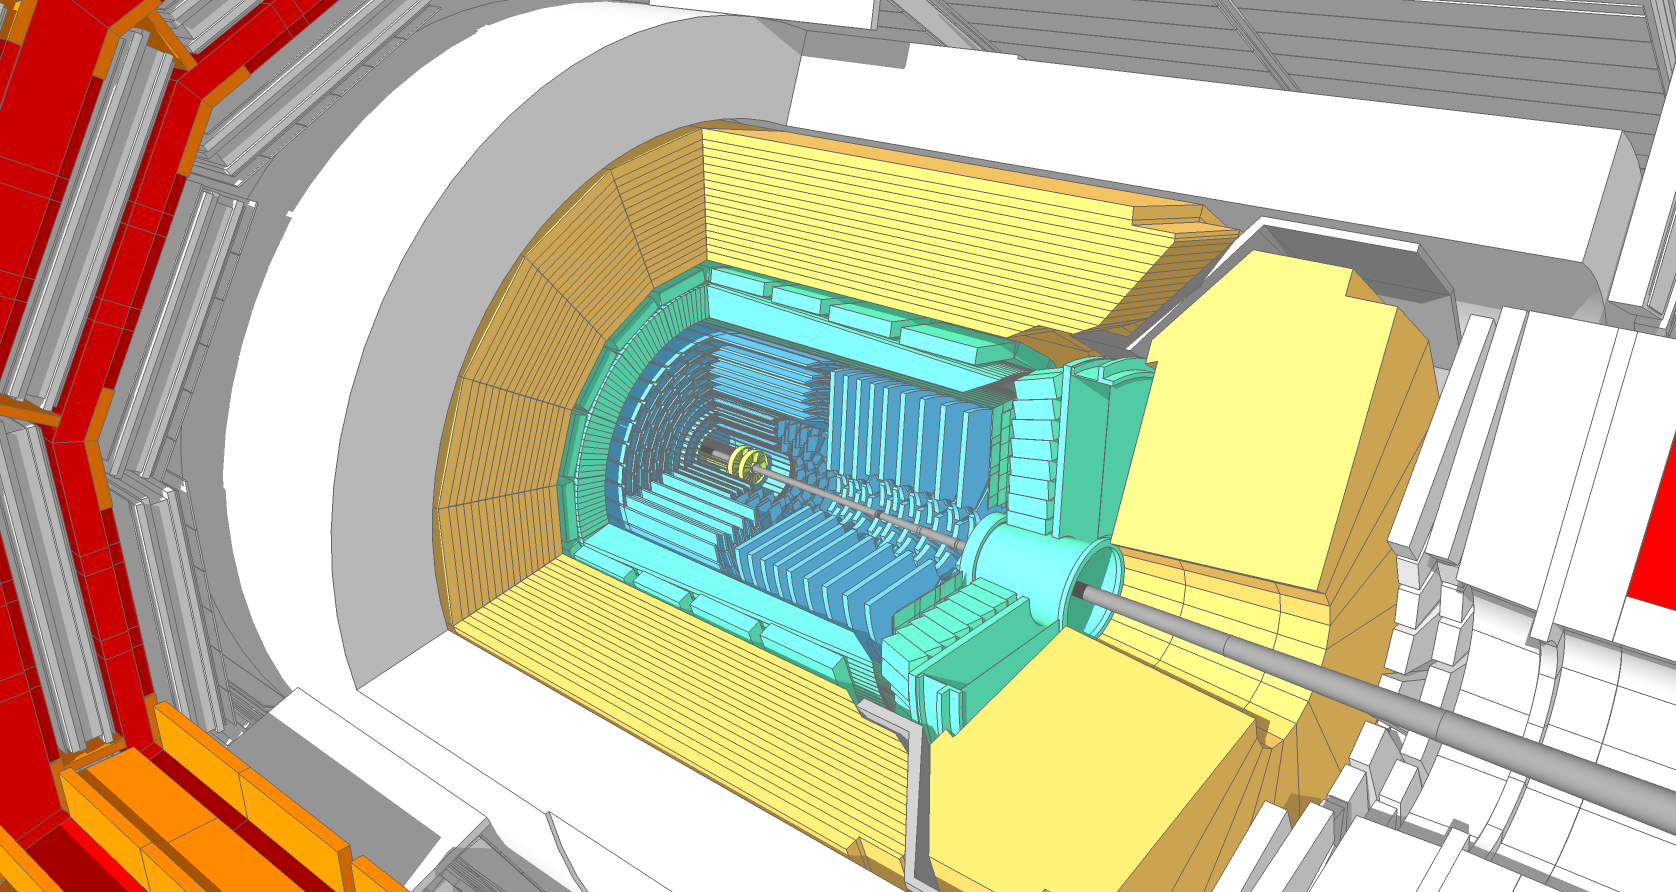
\includegraphics[width=0.8\textwidth]{hcal.png}
  \caption{Close up of the CMS calorimetry showing the ECAL (green) and the HCAL
(yellow) within the solenoid magnet (white).}
  \label{fig:calo}
\end{figure}

Lead tungstate crystals are ideally suited for this since the scintillation
decay time is similar to the LHC bunch crossing time, 
with \unit{80}{\%} of light being produced within \unit{25}{\ns}.
They also have a short radiation lengths ($X_0=\unit{0.89}{\cm}$) 
and Moliere length (\unit{2.2}{\cm}) as well as being radiation hard
(up to \unit{10}{\mrad}).

A disadvantage to using lead tungstate is that the light output of the crystals
is relatively low and changes with temperature. This is overcome by maintaining
a stable temperature (within \unit{0.1}{\degreecelsius}) and using
photodetectors with an intrinsic gain.
Silicon avalanche photodiodes (APDs) are used to detect the scintillation light
in the barrel and vacuum phototriodes (VPTs) are used in the endcap parts.

The barrel section of the ECAL (EB) surrounds the inner tracker. It is comprised
of 36 identical supermodules that each cover a half of the length of the barrel
($0<|\eta|<1.479$) and \unit{20}{\degree} in phi. Each supermodule contains
1700 crystals arranged in a $\phi - \eta$ grid with each crystal mounted in a
``semi-projective'' geometry, with each crystal alligned \unit{3}{\degree} off the
nominal interaction vertex. Each crystal has a cross-section of
\unit{$22 \times 22$}{\mm\squared} and a length of
\unit{230}{\mm} (\unit{25.8}{X_0}).

The endcaps (EE) are formed of two ``Dees'', semi-circular aluminium plates
which support the ``supercrystals'', 5x5 arrays of crystals. The crystals are
mounted off the nominal interaction vertex by a small angle in a similar way
to the barrel. 
Unlike the barrel the crystals are arranged in an x-y grid.
Installed in front of the endcap ECAL is a preshower system which allows for
the rejection of \Ppizero .\cite{cms}

\begin{figure}[htbp]
  \centering
  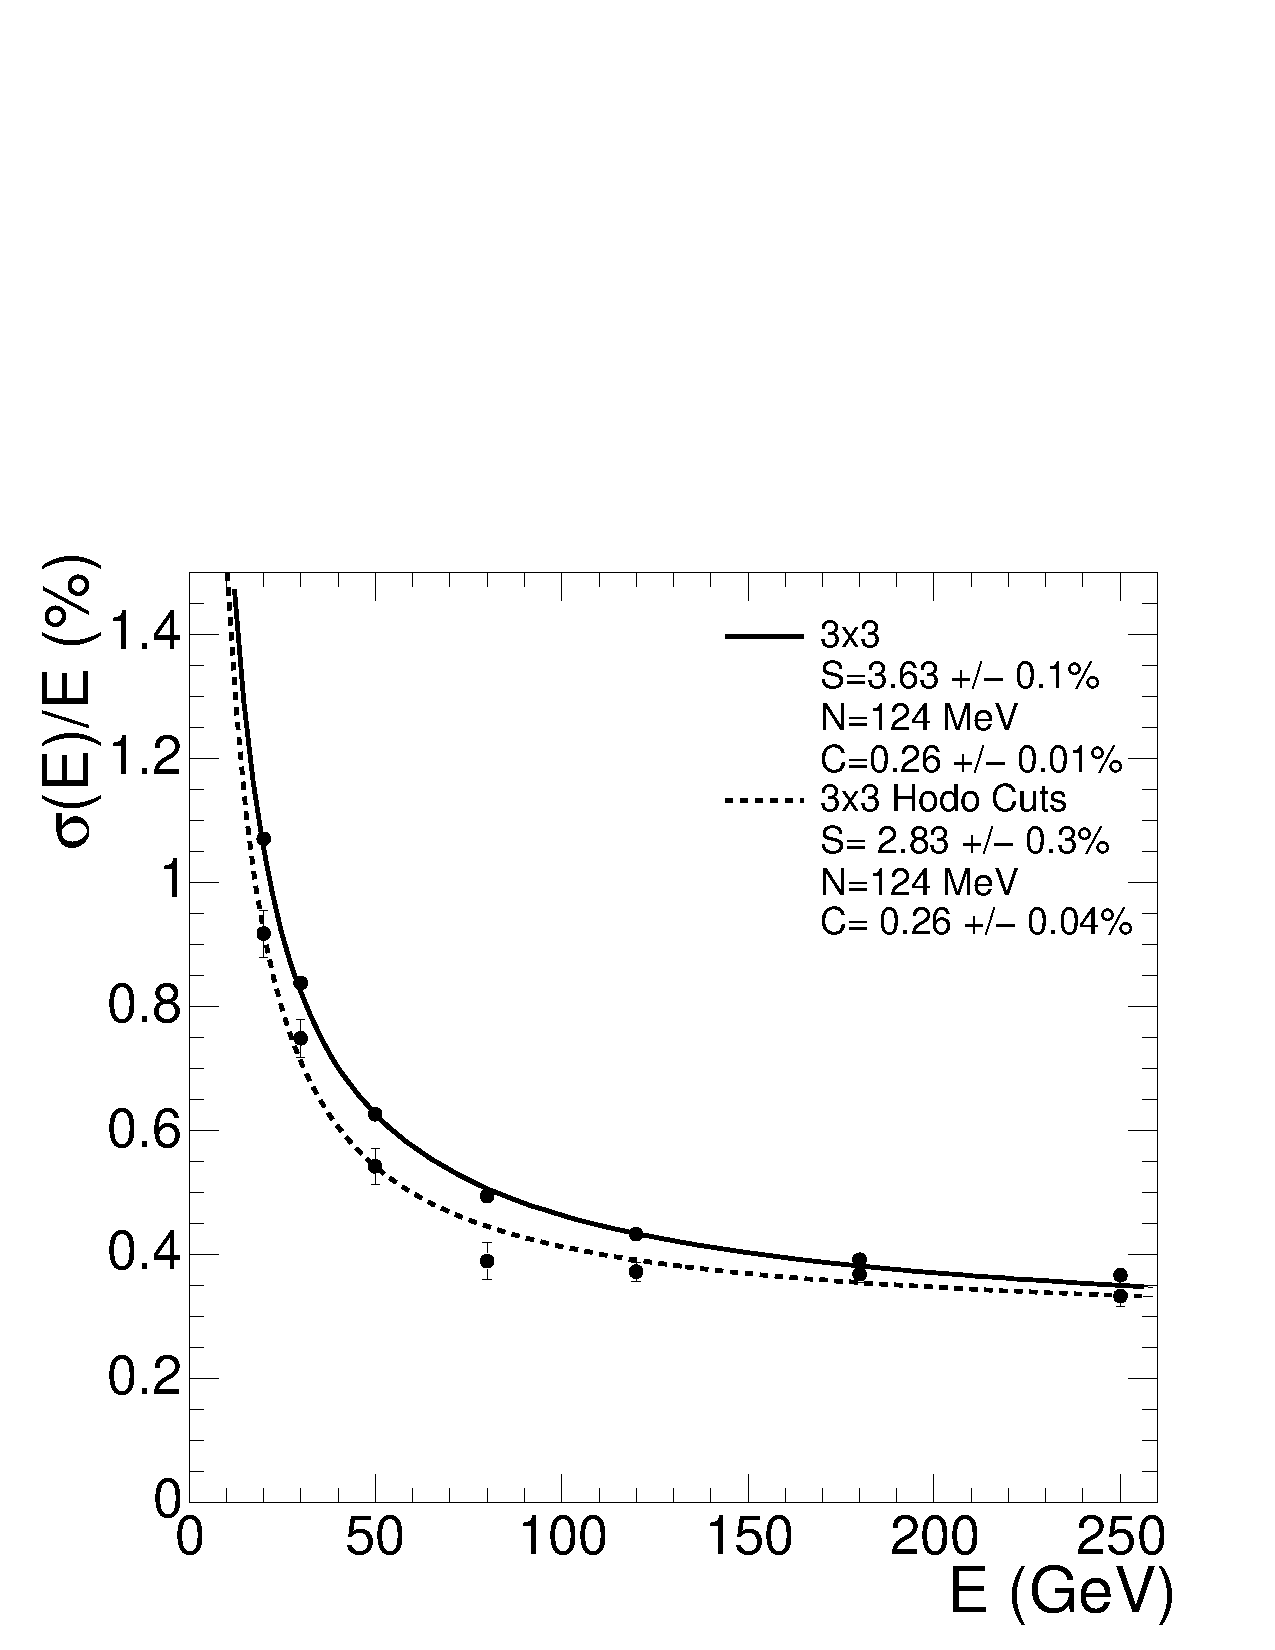
\includegraphics[width=0.6\textwidth]{ecal_performance}
  \caption{Energy resolution $\frac{\sigma}{E}$ of ECAL as a function of
  \label{fig:ECAL}
electron energy $E$. From \cite{cms}.}
\end{figure}

The ECAL energy resolution is shown in figure \ref{fig:ECAL} for test beam
electrons at several energies ($E$) and is fitted with the function
\begin{equation}
\left(\frac{\sigma}{E}\right)^{2} = \left(\frac{S}{\sqrt{E}}\right)^{2} +
\left(\frac{N}{E}\right)^{2} + C^{2}
\end{equation}
where S is the stochastic, N is the noise and C is the constant terms. The
stochastic term is due to the statistical fluctuations in the particles
produced in the electromagnetic shower. The noise term is due to electronic
noise and pile-up and is independent of energy. The constant term is due to
errors that are independent of energy, such as non-uniform signal generation
and calibration errors.\cite{cms}

% \subsubsection{ECAL Spikes!?}


% \subsubsection{ECAL Endcap Misalignment!?}
% It was found in early data taking that the ECAL endcaps are misaligned with
% respect to the tracker. This causes problems when reconstructing electrons
% since the difference between the track position and ECAL energy deposit is a
% variable that is cut on in the electron candidate selection. As a quick fix
% to this problem, an 

\subsection{Hadronic Calorimetry}

The Hadronic Calorimeter (HCAL) is designed to measure the energy of
hadron jets and the missing transverse energy (\met) which are important
signatures in many physics studies at the LHC.
A close up view of the CMS calorimetry is shown in \FigureRef{calo}, where the
HCAL is shown in yellow.

The HCAL is a brass/scintillator sampling hadron calorimeter that covers the
region up to $|\eta|<3.0$.
The scintillation light is channelled by wavelength shifting fibres, that are
embedded in the scintillation tiles, to hybrid photodiodes that can operate in
the high magnetic field. \cite{cms}

The HCAL comprises four components: the hadron barrel (HB), hadron outer (HO),
hadron endcap (HE) and the hadron forward (HF).

The hadron barrel covers the region ($|\eta| < 1.4$) and is positioned between
the ECAL and inside of the solenoid magnet coil
($\unit{1.77}{\meter}<R<\unit{2.95}{\meter}$).
This constrains the design of the HCAL and limits the total amount of material
to absorb the hadronic shower. 
To overcome this limitation the outer hadronic calorimeter is
placed outside the solenoid to complement the HCAL barrel and increases the
effective thickness of the hadron calorimetry to over 10 interaction lengths.

The hadron endcap covers the region $1.3 < |\eta| < 3.0$.
In the forward region ($|\eta| > 3$) energy measurements are made with an
iron/quartz-fibre forward hadronic calorimeter where the Cherenkov light is
detected by photodetectors. The calorimeter needs to be radiation hard 
due to the very large flux in the forward region.

\begin{figure}[htbp]
  \centering
  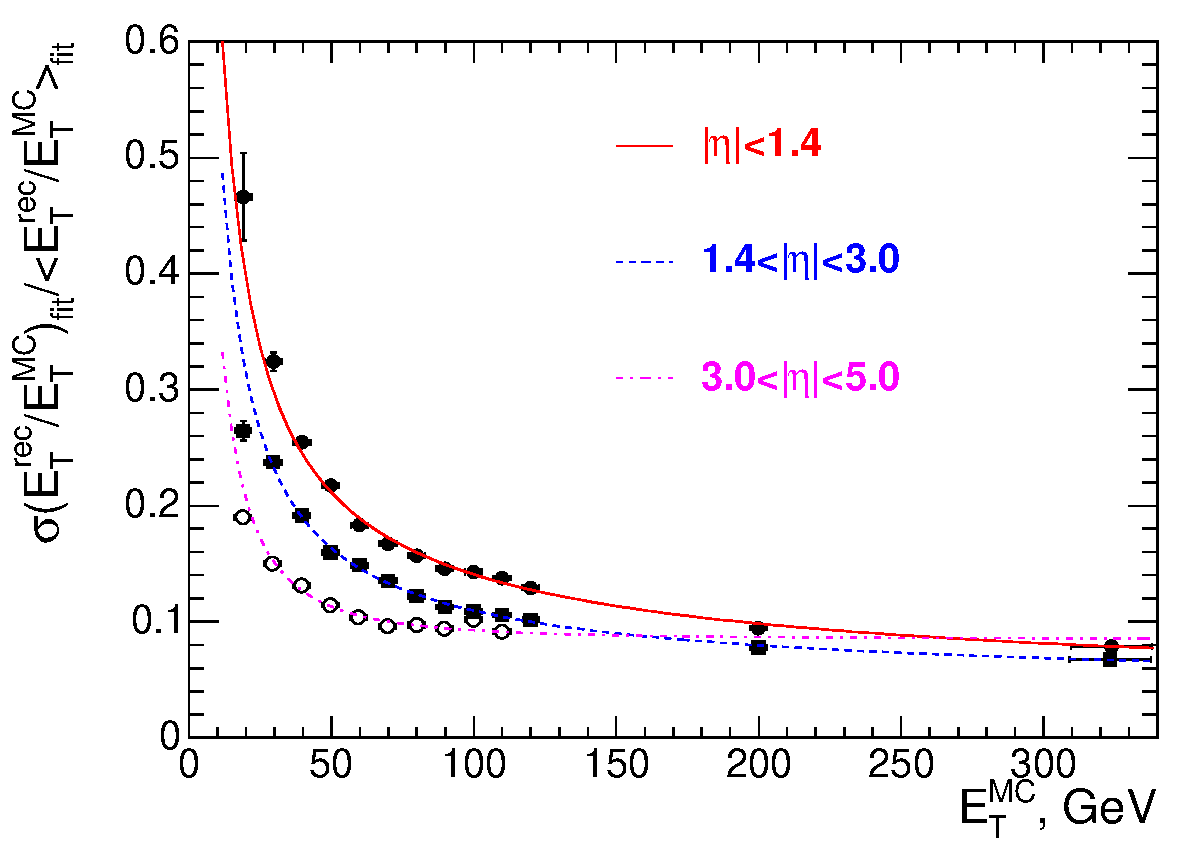
\includegraphics[width=0.45\textwidth]{hcal_performance}
  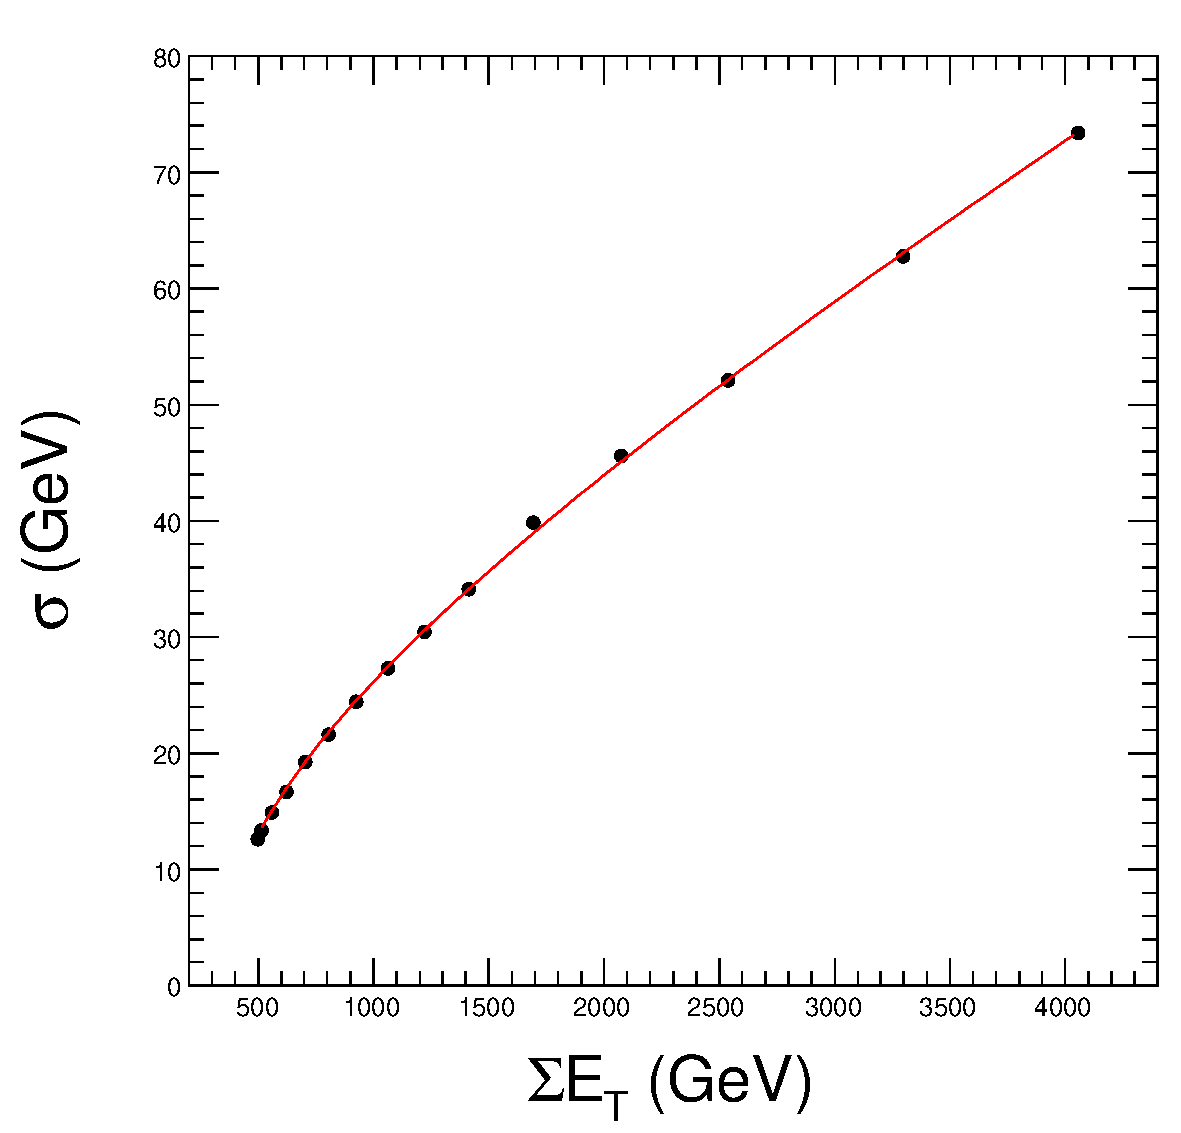
\includegraphics[width=0.45\textwidth]{met_res}
  \caption{Energy resolution $\frac{\sigma}{E}$ of HCAL as a function of jet
  \label{fig:HCAL}
transverse energy for barrel jets ($|\eta| < 1.4$), endcap jets ($1.4<|\eta| <
3$) and forward jets $3<|\eta| < 5$) (left)
Missing transverse energy resolution as a function of total transverse energy in
the event for QCD events with pile-up. (right). From \cite{cms}.}
\end{figure}

\FigureRef{fig:HCAL} shows the jet energy resolution as a function of jet
transverse energy for jets in each of the three regions. \FigureRef{fig:HCAL}
shows the missing transverse energy resolution as a function of the total jet
transverse energy in the event.

\subsection{Muon System}
The muon system lies outside of the CMS solenoid and the outer HCAL detectors.
It is designed to have three functions; to identify muons, measure the momentum
of muons and trigger on muons. To perform these functions the muon system
consists of several different types of detectors.

\begin{figure}[htbp]
  \centering
  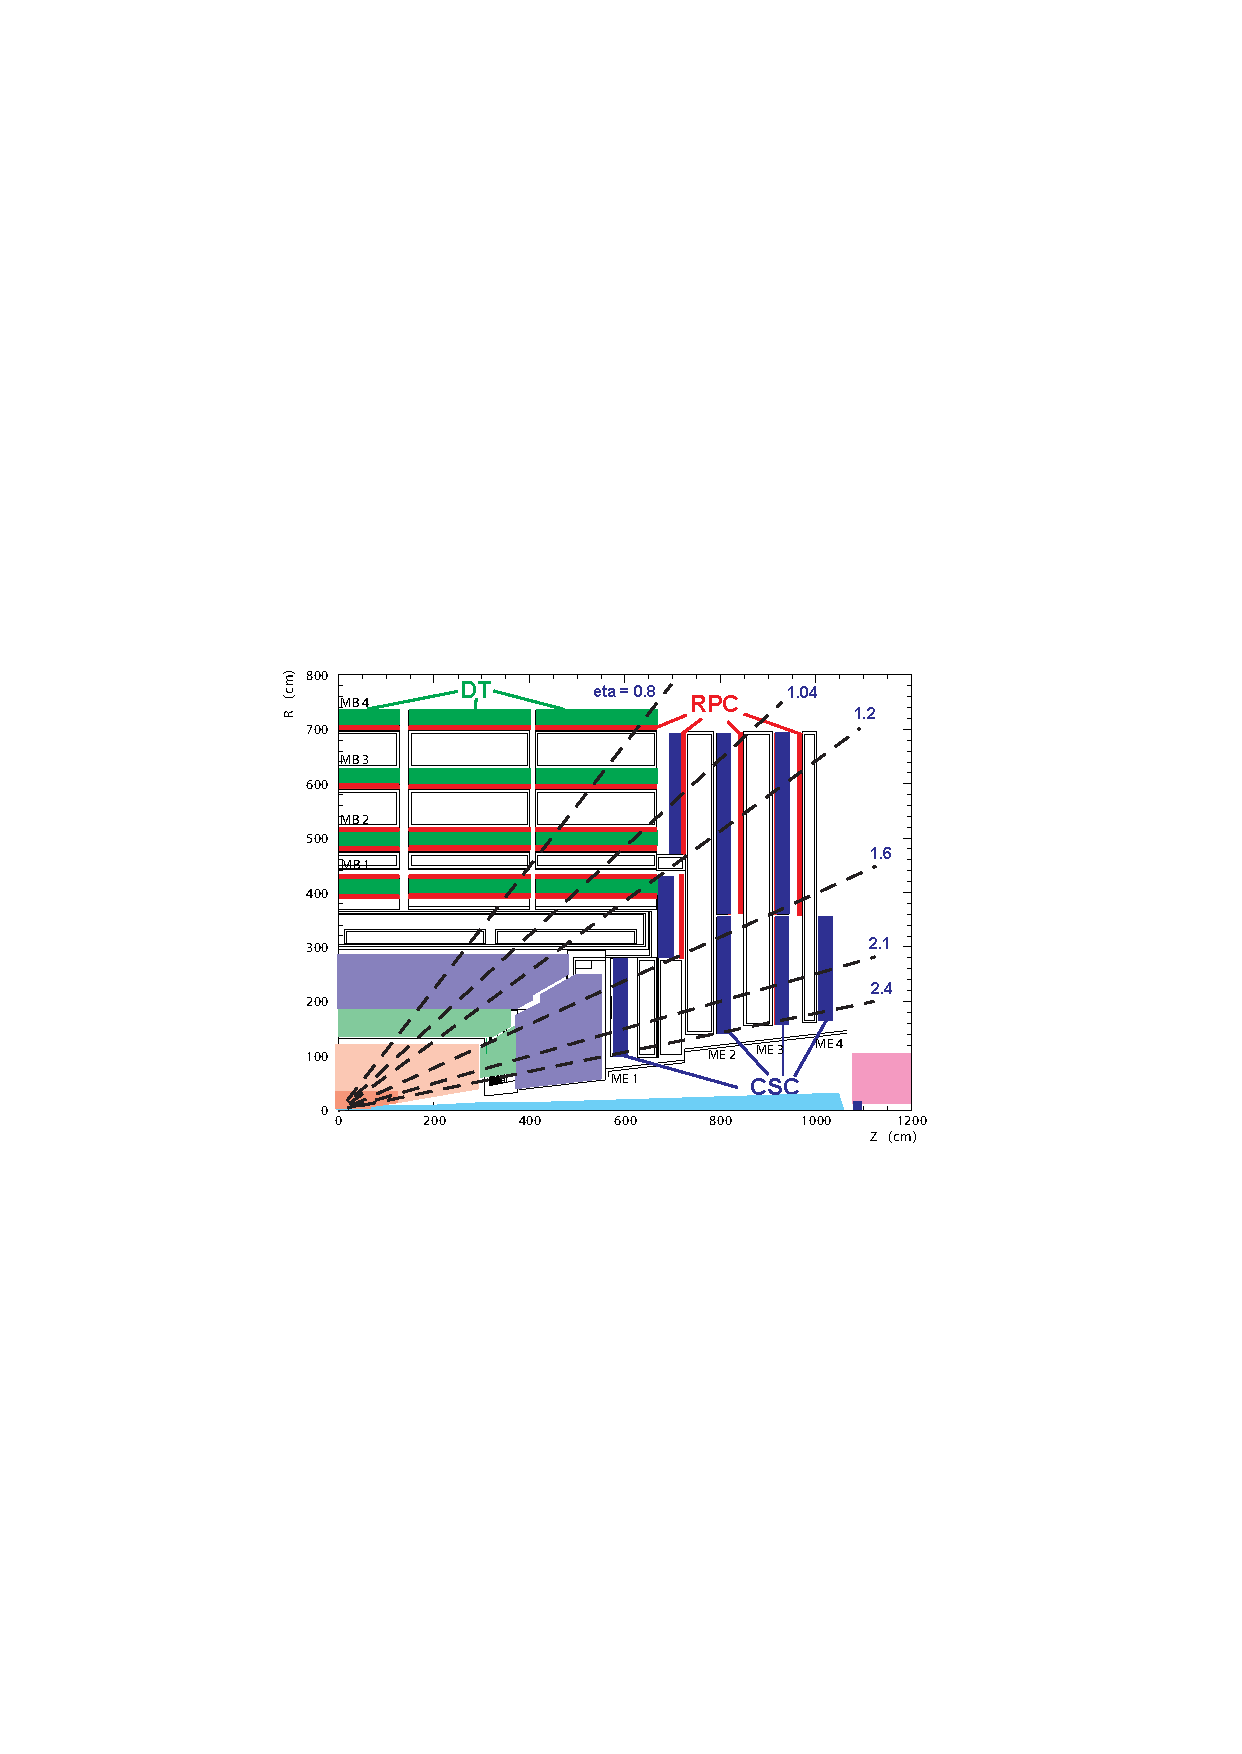
\includegraphics[width=0.8\textwidth]{muon_system}
  \caption{Muon system}
  \label{fig:muon_system}
\end{figure}

\subsubsection{Drift Tubes}
In the barrel region ($|\eta| < 1.2$) aluminium drift tubes (DT) are used
arranged in four stations interspersed along the layers of the flux return
plates. 
Each station contains 12 layers, eight to measure the coordinate in the
$r-\phi$ plane and four to measure the $z$ direction (except the fourth station
which only measures the $r-\phi$ plane). 

\subsubsection{Cathode Strip Chambers}
In the endcaps ($0.9<|\eta|<2.4$) cathode strip chambers (CSC) are used. The
CSCs are arranged in to four stations in each endcap arranged so they are
perpendicular to the beam line, and are placed between the flux return plates.
The cathode strips of each chamber run radially away from the beam line where
as the anode wires run perpendicular to the strips; both are read out which
gives information on both the $r-\phi$ plane (from the cathode) and the $\eta$
direction (from the anode). \cite{cms}

\subsubsection{Resistive Plate Chambers}
In addition to DT chambers and CSCs a complimentary trigger system is also used
consisting of resistive plate chambers (RPC) in the endcap and barrel regions.
The RPCs are able to provide a fast and independent trigger over a large range
($|\eta| < 1.6$). In the barrel region, 6 layers of RPCs are used, 2 in each of
the first 2 muon stations and 1 in each of the last 2 stations. In the endcap a
layer of RPCs in each of the first 3 stations.

An optical alignment system, that uses lasers and LEDs, measures the positions
of each muon station with respect to each other and the CMS inner tracker to
ensure an accurate and high resolution measurement of the muon
momentum.\cite{cms}

The performance of the muon system and inner tracker is shown in figure
\ref{fig:MS}.

\begin{figure}[htbp]
  \centering
  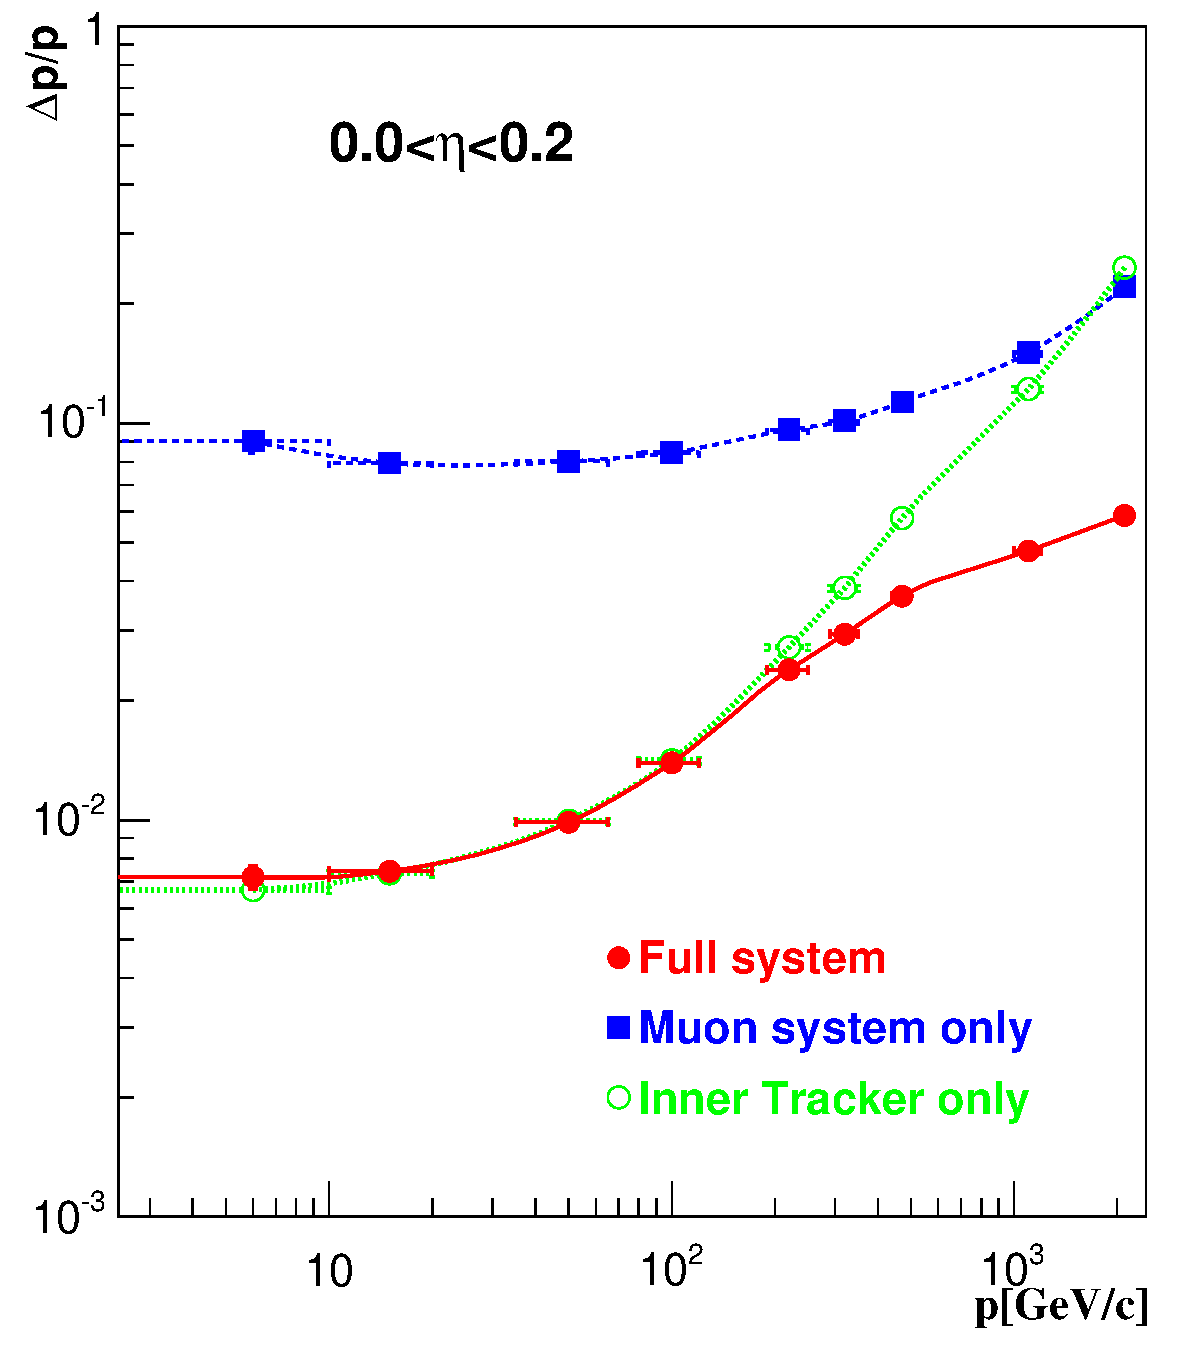
\includegraphics[width=0.45\textwidth]{muon_barrel}
  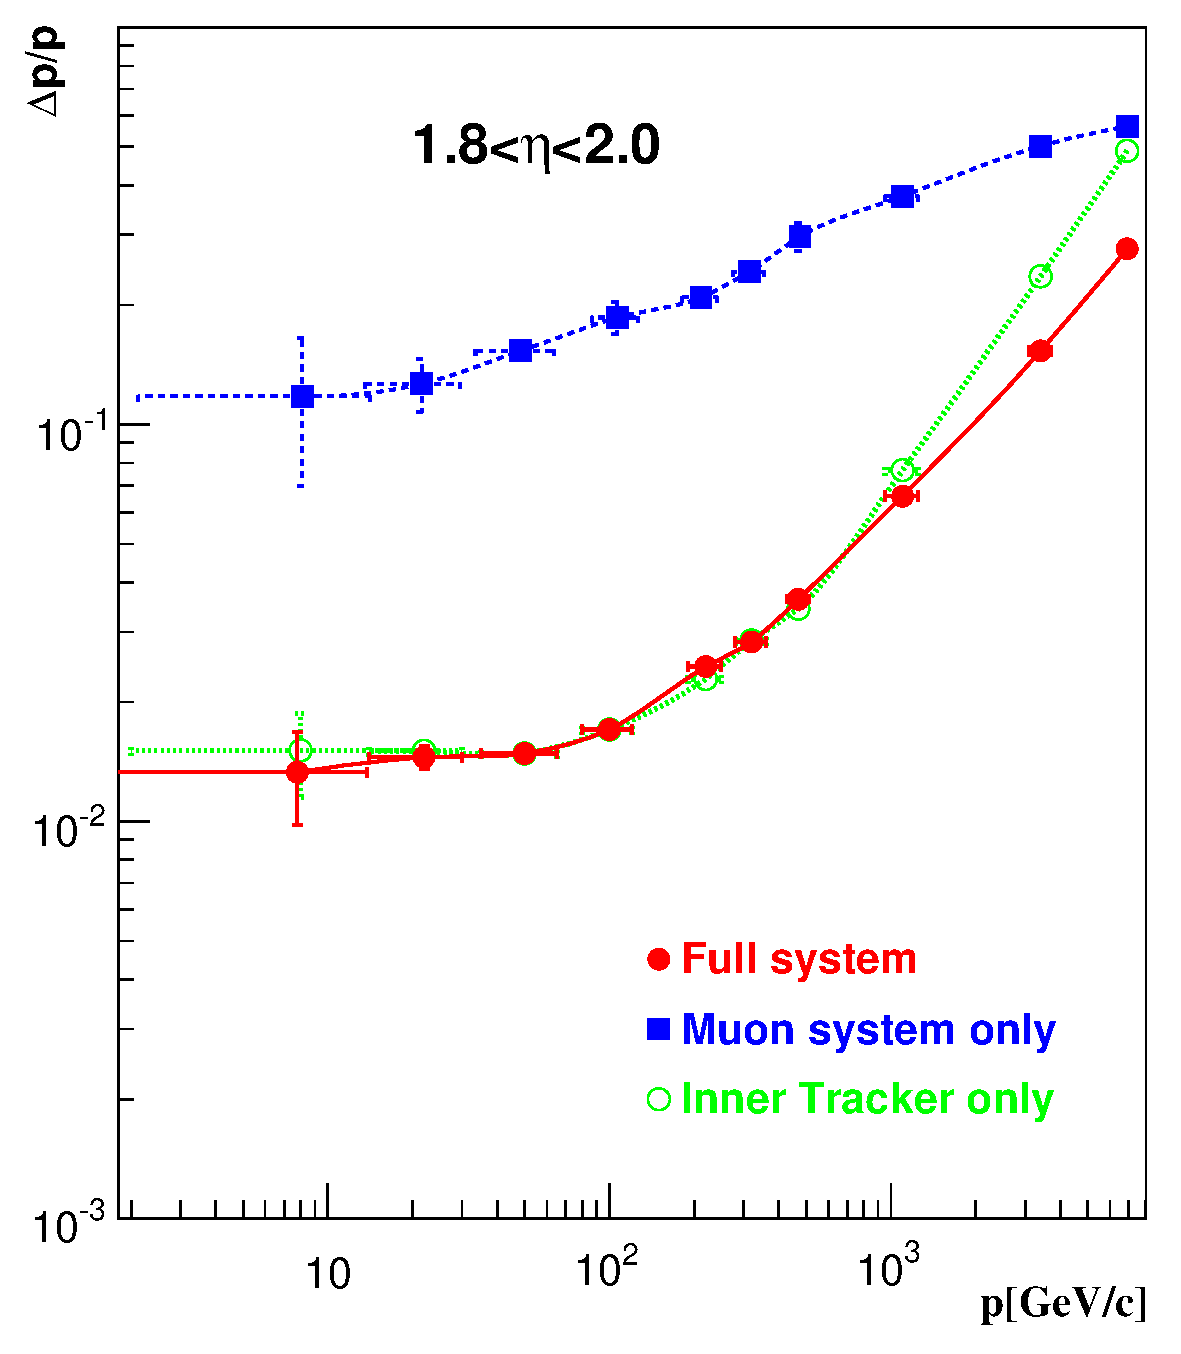
\includegraphics[width=0.45\textwidth]{muon_endcap}
  \caption{Muon transverse momentum resolution as a function of the
  \label{fig:MS}
transverse-momentum using only the muon system, only the tracker and both, for
left, barrel muons ($|\eta| < 0.8$) and right, endcap muons ($1.2<|\eta| <
2.4$). From \cite{cms}.}
\end{figure}


\subsection{Trigger and Data Acquisition}
At design luminosity, the high bunch crossing frequency of the LHC means that
CMS will observe a collision containing an average of 20 superimposed inelastic
events every \unit{25}{\nano\second}, a rate of $10^{9}$ interactions per
second.
A zero suppressed event output from CMS is about \unit{2}{\mega \bel} so the total data
output rate from CMS is \unit{$\approx 80$}{\tera \bel \per \second}
This is an unfeisable amount to store both in terms of the data capacity and the
rate at which the data will need to be written out.
In reality only about $\approx 10^{2}$ crossings can be written to the tape
storage every second. 

The vast majority of events will contain only inelastic collisions and not be of
interest from a physics perspective and can be discarded.  
It is the job of the trigger to reduce the rate of events
by a factor of $10^6$ by rejecting the uninteresting events while keeping as
many interesting events as possible.

An overview of the DAQ and trigger is shown in figure \ref{fig:CMSDAQ}.

\begin{figure}[htbp]
  \centering
  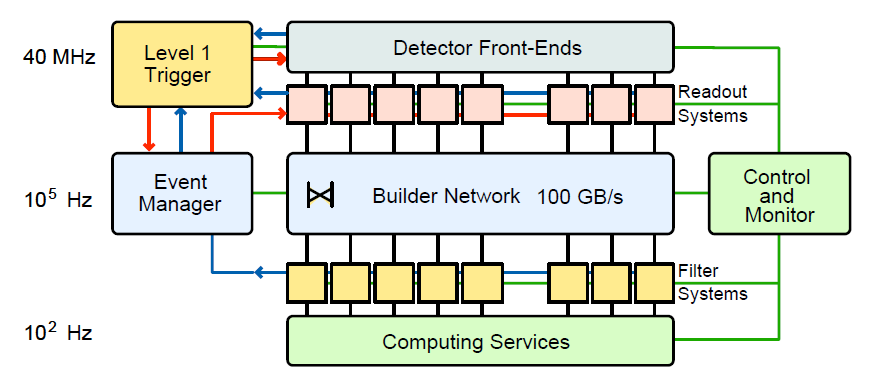
\includegraphics[width=0.6\textwidth]{CMSDAQ}
  \caption{Overview of the architecture of the CMS DAQ and trigger. From
  \label{fig:CMSDAQ}
\cite{cms}.}
\end{figure}

The trigger is separated in to two parts the Level-1 (L1) trigger and the High
Level Trigger (HLT).\cite{cms}

\subsubsection{Level-1 Trigger}

The Level-1 trigger (L1) is designed to reduce the event rate from the bunch
crossing frequency of \unit{40}{\mega\hertz} to a maximum output rate of
\unit{100}{\kilo\hertz}.
The L1 trigger is implemented with custom designed fast programmable electronics
 that takes as input coarsely segmented data from the calorimeters and muon systems and
places the high resolution data in pipelined memories. The reduced granularity
data is used to form ``trigger primatives'', such as electrons, photons muons
and jets that pass a certain \PT or \ET threshold, which the L1 Trigger uses to
base its decision. It also recieves information on event wide variables such as
the total sum of transverse energy and the missing transverse energy.

\subsubsection{High-Level Triggers}
After a fixed time interval of \unit{3.2}{\micro\second} the high resolution
event data held in the memory pipelines is either readout or discarded depending
the decision at the Level-1 trigger. For a proton-proton event
the data is about \unit{1.5}{\mega\bel} in size.
The data is transfered to a processor running the high-level trigger software.

The high-level trigger (HLT) is a software system which runs on a server farm with
over one thousand commercial multicore processors with access to the complete
event data allowing it to make more complex calculations. 
Objects are reconstructed in the HLT as they are needed and events are discarded
as soon as possible to avoid wasted processing time.

Events that pass the triggers are sent to Tier-0 storage where they are
undergo reconstruction. The data is then distributed to Tier-1 and Tier-2 sites
at laboratories and universities around the world.

